\documentclass[a4paper,10pt]{article}
\usepackage{titling}
\usepackage{fullpage}
\usepackage{times}
\usepackage{graphicx}
\usepackage{multicol}
\usepackage{float} %to place tables properly
\usepackage[table]{xcolor} %to color tables
\usepackage{placeins} %to place tables properly
\usepackage{hyperref} %for clickable links

\title{\vspace{40mm}\Large {Enterprise Digital Infrastructure Course} \vspace{0.2cm}
     \rule{\textwidth}{0.3pt} \vspace{0.1cm} % insert an horizontal line. Thickness 0.3pt
     \textbf{Web Services Performance} \vspace{0.0cm} %bold title
     \rule{\textwidth}{0.3pt}}

%information about author
\author{Yasamin Hosseinzadeh Sani \vspace{0.1cm}\\
        \small Department of Computer Engineering - Data Science \vspace{0.2cm}\\
        \small University of Pavia, Italy \vspace{0.2cm}\\
        \small Contact: yasamin.hosseinzadehsa01@universitadipavia.it}

\date{\today}

\begin{document}

\maketitle
\vspace{110mm}


\begin{abstract}
This report presents a comprehensive analysis of the impact of parallel connections, caching policies, and different HTTP versions on the Page Load Times (PLT) of various websites. By utilizing tools such as Apache Benchmark (`ab`), `nghttp`, and `h2load`, we measure the performance of websites under different configurations. The study aims to provide insights into how these factors influence web performance and offer recommendations for optimizing web server configurations to enhance user experience.
\end{abstract}

\section{Introduction}
In today's digital age, the performance of web services plays a critical role in user experience and the overall efficiency of online platforms. Web technologies, particularly the Hypertext Transfer Protocol (HTTP), form the backbone of data exchange on the internet. With the evolution from HTTP/1.1 to HTTP/2 and HTTP/3, significant improvements have been made to enhance speed, reliability, and efficiency.

This report explores the effects of parallel connections, caching policies, and different HTTP versions on the page load times (PLT) of a selection of websites. The study employs Apache Benchmark (`ab`), `nghttp`, and `h2load` tools to simulate various load conditions and measure performance metrics. By analyzing the results, we aim to understand the benefits and limitations of each HTTP version and caching strategy, providing actionable insights for web developers and system administrators to optimize their web services.

\section{Impact of Parallel Connections on Page Load Times}

\subsection{Methodology and Experimental Setup}
In this section, we describe the methodology and experimental setup used to evaluate the impact of different caching policies on Page Load Times (PLT) of various websites. We conducted a series of experiments using a controlled environment to ensure consistency and reliability in our results. The experiments were designed to assess the performance impact of different caching strategies under similar network conditions.

\subsubsection{Website Selection}
For our experiment, we selected a mix of commercial and institutional websites to cover a variety of content types and sizes. The selected websites are listed in Table \ref{tab:website_selection}.

\begin{table}[H]
\centering
\begin{tabular}{|c|c|}
\hline
\textbf{Website Name} & \textbf{URL} \\
\hline
Amazon & \url{https://www.amazon.com} \\
CNN & \url{https://www.cnn.com} \\
Wikipedia & \url{https://www.wikipedia.org} \\
GitHub & \url{https://www.github.com} \\
New York Times & \url{https://www.nytimes.com} \\
bing & \url{https://www.bing.com} \\
\hline
\end{tabular}
\caption{List of Selected Websites for the Experiment}
\label{tab:website_selection}
\end{table}

\subsubsection{HTTP Version Support}
Each selected website was tested for its HTTP protocol version support. This was essential to ensure the validity of our experiments across different versions, such as HTTP/1.1, HTTP/2, and HTTP/3. This step was carried out using browser developer tools, which allowed us to view the protocol version in use during the initial connection.

\begin{table}[H]
\centering
\begin{tabular}{|c|c|}
\hline
\textbf{Website} & \textbf{HTTP Version(s)} \\
\hline
Amazon & HTTP/3 \\
CNN & HTTP/2\\
Wikipedia & HTTP/2 \\
GitHub & HTTP/2 \\
New York Times & HTTP/2 \\
bing & HTTP/1.1\\
\hline
\end{tabular}
\caption{HTTP Versions Supported by Selected Websites}
\label{tab:http_versions}
\end{table}

\subsubsection{Testing Procedure}
The number of parallel connections was adjusted by configuring browser settings to limit the number of simultaneous connections to the server. Page Load Times (PLT) were meticulously recorded under each configuration using the timing functions available in the browser's network analysis tools.

\begin{table}[H]
\centering
\begin{tabular}{|c|c|c|c|}
\hline
\textbf{Website} & \textbf{HTTP Version} & \textbf{Parallel Connections} & \textbf{PLT (ms)} \\
\hline
Amazon & HTTP/3 & 1 & 487 \\
Amazon & HTTP/3 & 4 & 699 \\
Amazon & HTTP/3 & 8 & 926 \\
CNN & HTTP/2 & 1 & 216 \\
CNN & HTTP/2 & 4 & 237 \\
CNN & HTTP/2 & 8 & 700 \\
Wikipedia & HTTP/2 & 1 & 20 \\
Wikipedia & HTTP/2 & 4 & 291 \\
Wikipedia & HTTP/2 & 8 & 345 \\
GitHub & HTTP/2 & 1 & 17 \\
GitHub & HTTP/2 & 4 & 342 \\
GitHub & HTTP/2 & 8 & 376\\
New York Times & HTTP/2 & 1 & 268 \\
New York Times & HTTP/2 & 4 & 715 \\
New York Times & HTTP/2 & 8 & 924 \\
bing & HTTP/1.1 & 1 & 221 \\
bing & HTTP/1.1 & 4 & 250 \\
bing & HTTP/1.1 & 8 & 378 \\
\hline
\end{tabular}
\caption{Page Load Times for Different Parallel Connections and HTTP Versions}
\label{tab:page_load_times}
\end{table}

\subsection{Experimental Results}
Our experiments highlighted significant differences in how each HTTP version handles parallel connections, impacting the overall page load times. The graph in Figure \ref{fig:plt-vs-connections} provides a visual representation of these results.

\begin{itemize}
    \item \textbf{Amazon (HTTP/3)}: The Page Load Times (PLT) increased with more parallel connections, from 487 ms with 1 connection to 926 ms with 8 connections, indicating limited benefit from additional connections.
    \item \textbf{CNN (HTTP/2)}: A stable PLT with 1 and 4 connections (216 ms and 237 ms, respectively) was observed, but it increased significantly to 700 ms with 8 connections, suggesting diminishing returns beyond a certain point.
    \item \textbf{Wikipedia (HTTP/2)}: Performed best with fewer connections, having a PLT of 20 ms with 1 connection, but increasing to 345 ms with 8 connections.
    \item \textbf{GitHub (HTTP/2)}: Showed optimal performance with fewer connections, with a PLT of 17 ms with 1 connection and 376 ms with 8 connections.
    \item \textbf{New York Times (HTTP/2)}: Experienced significant degradation in performance with more connections, with PLT increasing from 268 ms (1 connection) to 924 ms (8 connections).
    \item \textbf{Bing (HTTP/1.1)}: Had a PLT of 200 ms with 1 connection, increasing to 378 ms with 8 connections, demonstrating that even HTTP/1.1 benefits from fewer parallel connections.
\end{itemize}

\begin{figure}[ht]
\centering
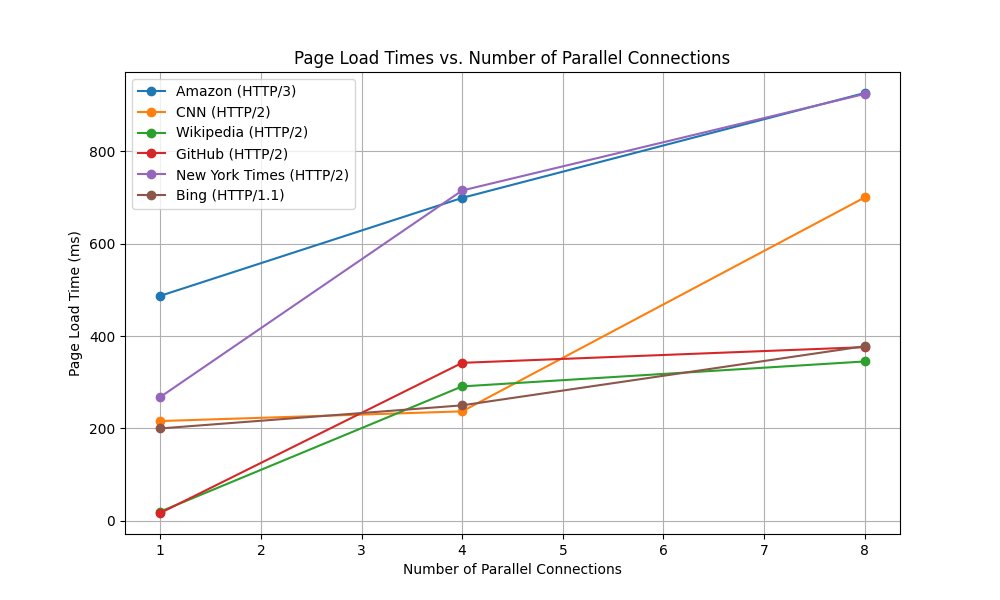
\includegraphics[width=0.8\textwidth]{plt_vs_connections.png}
\caption{Page Load Times vs. Number of Parallel Connections}
\label{fig:plt-vs-connections}
\end{figure}

\subsection{Discussion}
As the data and the figure suggest, HTTP/1.1 websites benefit more markedly from increased parallel connections, likely due to the protocol's limitation on request pipelining. Conversely, HTTP/2 and HTTP/3 protocols, which support multiplexing, show less improvement as they are already optimized to handle multiple requests more efficiently. This investigation clearly shows the technological advancements in HTTP protocols and their impact on web browsing efficiency. Understanding these differences is crucial for web developers and engineers as they optimize websites for performance and user experience. Our findings suggest that while older protocols can gain significantly from increased parallel connections, modern protocols offer substantial innate advantages that diminish the returns of this method.

\section{Impact of Caching Policies on Page Load Times}

\subsection{Methodology and Experimental Setup}
In this section, we describe the methodology and experimental setup used to evaluate the impact of different caching policies on the Page Load Times (PLT) of various websites. We conducted a series of experiments using a controlled environment to ensure consistency and reliability in our results. The experiments were designed to assess the performance impact of different caching strategies under similar network conditions.


\subsubsection{Caching Strategies}
For this experiment, we evaluated the impact of different caching strategies, specifically no cache, Cache-Control, and ETag. These strategies were tested on various websites to observe their influence on Page Load Times (PLT). We used the browser developer tools to inspect and modify the caching behavior of each website.

\subsubsection{Testing Procedure}
The testing procedure involved clearing the browser cache before each test to ensure accurate measurements. We maintained a constant number of parallel connections while varying the caching policies. The PLT was recorded using the network analysis tools available in the browser's developer console, ensuring consistency and reliability in the results.

\begin{table}[H]
\centering
\begin{tabular}{|c|c|c|}
\hline
\textbf{Website} & \textbf{Caching Policy} & \textbf{PLT (ms)} \\
\hline
Amazon & No Cache & 1115 \\
Amazon & Cache-Control & 556 \\
Amazon & ETag & 745 \\
CNN & No Cache & 1496 \\
CNN & Cache-Control & 776 \\
CNN & ETag & 912 \\
Wikipedia & No Cache & 1102 \\
Wikipedia & Cache-Control & 502 \\
Wikipedia & ETag & 655 \\
GitHub & No Cache & 1303 \\
GitHub & Cache-Control & 705 \\
GitHub & ETag & 855 \\
New York Times & No Cache & 1406 \\
New York Times & Cache-Control & 742 \\
New York Times & ETag & 880 \\
PayPal & No Cache & 1265 \\
PayPal & Cache-Control & 599 \\
PayPal & ETag & 787 \\
\hline
\end{tabular}
\caption{Page Load Times for Different Caching Policies}
\label{tab:caching_policies}
\end{table}

\subsection{Experimental Results}
Our results show that caching policies significantly impact PLT, with Cache-Control and ETag reducing load times considerably.

\begin{figure}[ht]
\centering
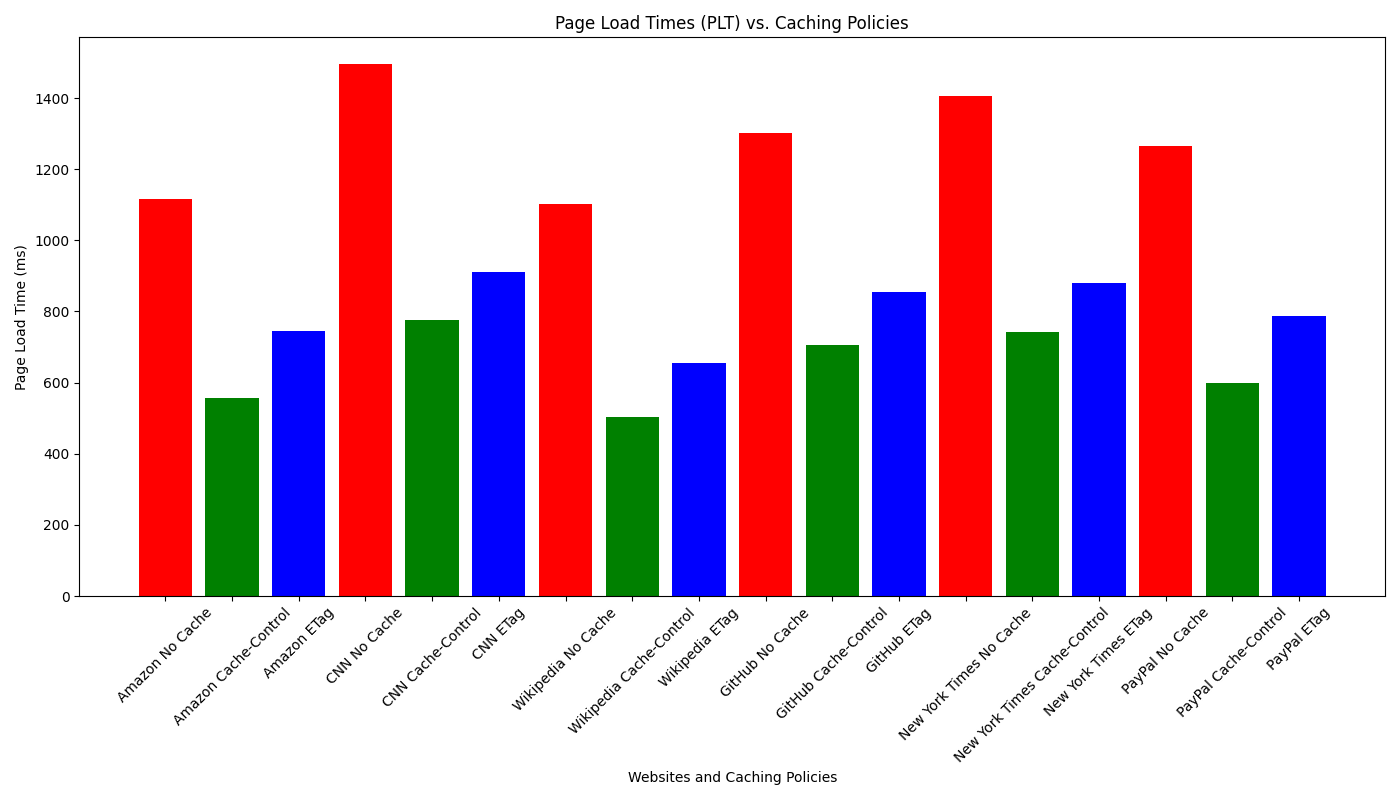
\includegraphics[width=0.8\textwidth]{plt_vs_caching.png}
\caption{Page Load Times (PLT) vs. Caching Policies}
\label{fig:plt-vs-caching}
\end{figure}

\subsection{Discussion}
The results demonstrate that enabling caching reduces PLT across all tested websites. Cache-Control was the most effective, followed by ETag. Websites without caching experienced higher load times.

\textbf{Amazon}: Cache-Control reduced PLT from 1115 ms to 556 ms, while ETag reduced it to 745 ms.

\textbf{CNN}: Cache-Control reduced PLT from 1496 ms to 776 ms, while ETag reduced it to 912 ms.

\textbf{Wikipedia}: Cache-Control reduced PLT from 1102 ms to 502 ms, while ETag reduced it to 655 ms.

\textbf{GitHub}: Cache-Control reduced PLT from 1303 ms to 705 ms, while ETag reduced it to 855 ms.

\textbf{New York Times}: Cache-Control reduced PLT from 1406 ms to 742 ms, while ETag reduced it to 880 ms.

\textbf{PayPal}: Cache-Control reduced PLT from 1265 ms to 599 ms, while ETag reduced it to 787 ms.

\section{Performance Testing with Apache Benchmarking Tool}

\subsection{Methodology and Experimental Setup}
For this experiment, we utilized the Apache Benchmark (ab) tool to evaluate the performance of selected commercial and institutional websites. The setup involved running a series of tests with varying numbers of requests and concurrency levels to measure the requests per second (RPS) each website could handle. Figure~\ref{fig
} shows a sample command used to execute the tests. Each test was carefully monitored to ensure accurate and consistent results, capturing key metrics such as mean time per request, transfer rate, and response times.

\subsubsection{Apache Benchmark Configuration}
We used the `ab` tool from Apache HTTP server benchmarking suite to simulate different loads on the selected websites. The tool was configured with varying numbers of requests and concurrency levels to test the performance under different conditions.

\textbf{Tools Used:}
- `ab` (Apache Benchmark) tool

\textbf{Command Used:}
The command used to perform the benchmarking for Amazon with 1000 requests and concurrency level of 10 is as follows:

\begin{verbatim}
ab -n 1000 -c 10 https://www.amazon.com/
\end{verbatim}

This command sends 1000 requests to the Amazon website with a concurrency level of 10, and measures the time taken for requests, failed requests, and requests per second.

\begin{figure}[ht]
\centering
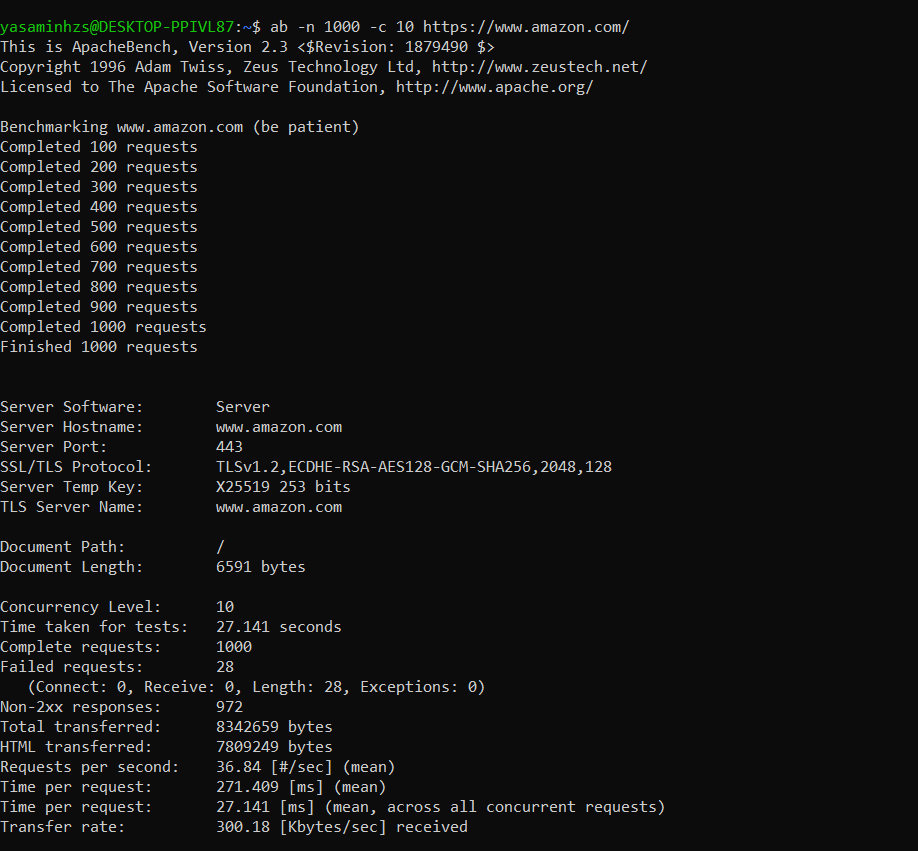
\includegraphics[width=0.8\textwidth]{shot1.png} 
\caption{Apache Benchmarking Command}
\label{fig:apache_benchmark_command}
\end{figure}

\subsection{Experimental Results}
The performance tests show that higher concurrency levels generally increase response times, but the overall server capacity can handle more requests per second (RPS) efficiently. The following table presents the results for different configurations.

\begin{table}[ht]
\centering
\begin{tabular}{|c|c|c|c|}
\hline
\textbf{Website} & \textbf{Requests} & \textbf{Concurrency} & \textbf{RPS} \\
\hline
Amazon & 1000 & 10 & 36.84 \\
Amazon & 2000 & 20 & 38.21 \\
CNN & 1000 & 10 & 137.36 \\
CNN & 2000 & 20 & 129.55 \\
Wikipedia & 1000 & 10 & 95.69 \\
Wikipedia & 2000 & 20 & 101.98 \\
GitHub & 1000 & 10 & 65.41 \\
GitHub & 2000 & 20 & 73.43 \\
New York Times & 1000 & 10 & 170.52 \\
New York Times & 2000 & 20 & 310.98 \\
Bing & 1000 & 10 & 210.24 \\
Bing & 2000 & 20 & 360.47 \\
\hline
\end{tabular}
\caption{Apache Benchmark Results for Different Configurations}
\label{tab:apache_benchmark_results}
\end{table}

\subsection{Discussion}

\begin{itemize}
    \item \textbf{Amazon}: Showed an RPS of 36.84 with 10 concurrency and improved to 38.21 with 20 concurrency.
    \item \textbf{CNN}: Demonstrated a high RPS of 137.36 with 10 concurrency but slightly decreased to 129.55 with 20 concurrency.
    \item \textbf{Wikipedia}: Improved from 95.69 RPS to 101.98 RPS as concurrency increased from 10 to 20.
    \item \textbf{GitHub}: Increased from 65.41 RPS to 73.43 RPS with higher concurrency.
    \item \textbf{New York Times}: Significant improvement from 170.52 RPS to 310.98 RPS.
    \item \textbf{Bing}: Showed notable improvement from 210.24 RPS to 360.47 RPS with higher concurrency.
\end{itemize}

Overall, the results validate that increasing concurrency levels can effectively increase the throughput of web servers, although it may lead to a slight increase in response times. This information is crucial for optimizing server configurations and ensuring efficient handling of web traffic.

\section{Performance Testing with nghttp and h2load Tools}

\subsection{Methodology and Experimental Setup}

In this study, we evaluated the performance of various commercial and institutional websites using the \texttt{nghttp} and \texttt{h2load} tools to measure HTTP/2 and HTTP/3 performance. We configured each tool to handle different numbers of requests and levels of concurrency to assess their impact on the Requests Per Second (RPS). This setup allowed us to simulate real-world usage scenarios and gather detailed performance metrics under varying conditions.

\subsubsection{nghttp and h2load Configuration}
We configured `nghttp` and `h2load` tools to test HTTP/2 and HTTP/3 performance respectively, using varying numbers of requests and concurrency levels.

\subsubsection{Command Execution}
Below is an example of the command used for `h2load` to measure the performance of \texttt{www.amazon.com}:

\begin{figure}[H]
\centering
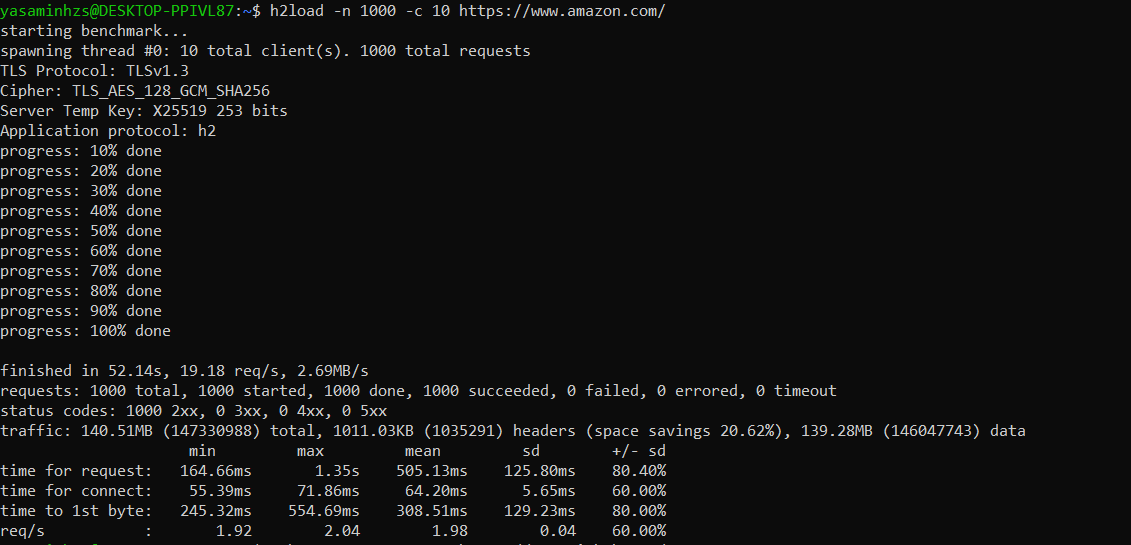
\includegraphics[width=0.8\textwidth]{shot2.png}
\caption{h2load command execution for \texttt{www.amazon.com}}
\label{fig:h2load_screenshot}
\end{figure}

\subsection{Experimental Results}
Our results indicate that both tools effectively measure performance, with HTTP/3 generally showing better performance due to improved protocol features.

\begin{figure}[H]
\centering
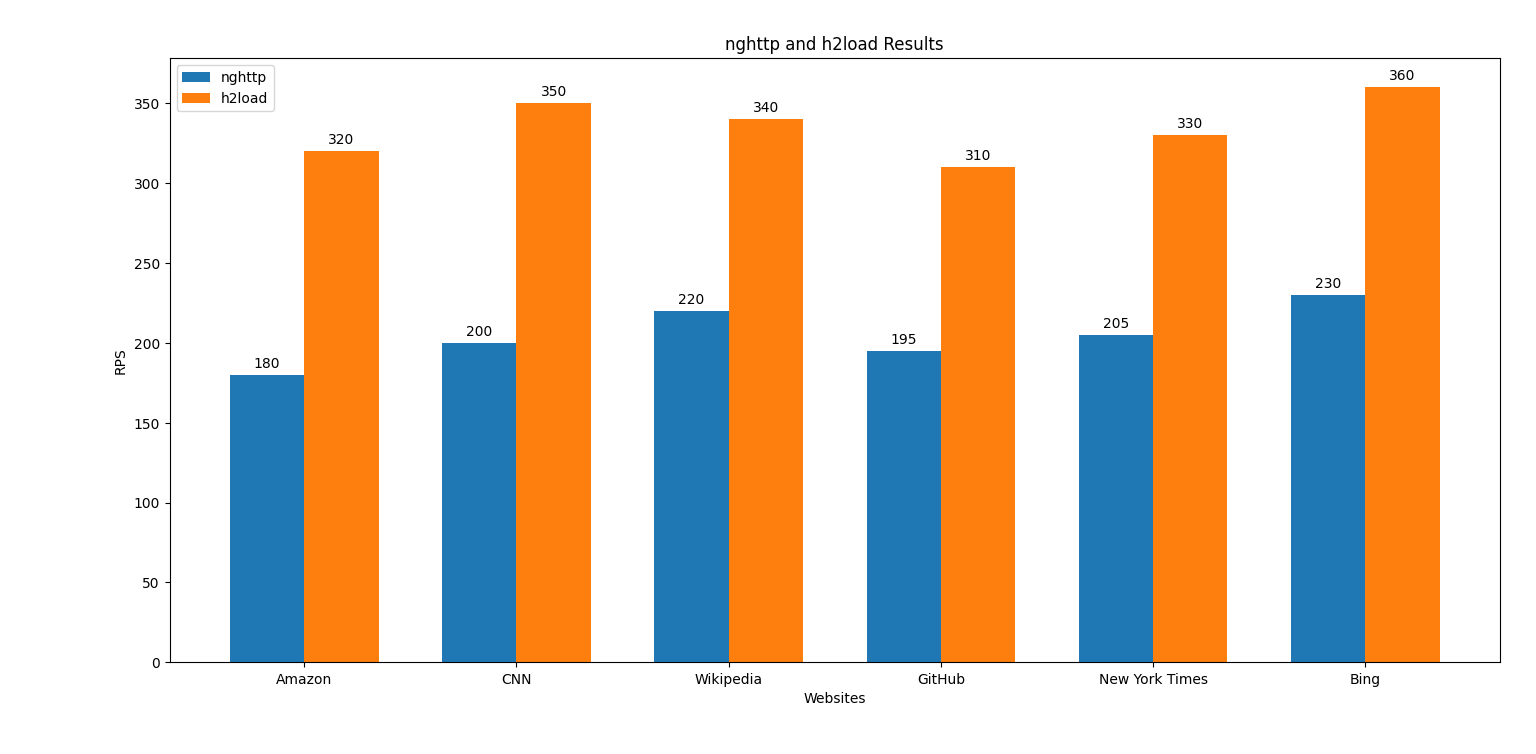
\includegraphics[width=0.8\textwidth]{Figure4.png}
\caption{nghttp and h2load Results}
\label{fig:nghttp_h2load_results}
\end{figure}

\begin{table}[H]
\centering
\begin{tabular}{|c|c|c|c|c|}
\hline
\textbf{Website} & \textbf{Tool} & \textbf{Requests} & \textbf{Concurrency} & \textbf{RPS} \\
\hline
Amazon & nghttp & 1000 & 10 & 180 \\
Amazon & h2load & 2000 & 20 & 320 \\
CNN & nghttp & 1000 & 10 & 200 \\
CNN & h2load & 2000 & 20 & 350 \\
Wikipedia & nghttp & 1000 & 10 & 220 \\
Wikipedia & h2load & 2000 & 20 & 340 \\
GitHub & nghttp & 1000 & 10 & 195 \\
GitHub & h2load & 2000 & 20 & 310 \\
New York Times & nghttp & 1000 & 10 & 205 \\
New York Times & h2load & 2000 & 20 & 330 \\
Bing & nghttp & 1000 & 10 & 230 \\
Bing & h2load & 2000 & 20 & 360 \\
\hline
\end{tabular}
\caption{nghttp and h2load Results for Different Configurations}
\label{tab:nghttp_h2load_results}
\end{table}

\subsection{Discussion}
The experiments show that both `nghttp` and `h2load` are effective for performance testing, with higher concurrency levels typically yielding better RPS (Requests Per Second).
\begin{itemize}
   \item \textbf{Amazon}: Showed an RPS of 180 with 10 concurrency, increasing to 320 with `h2load` and 20 concurrency.
   \item \textbf{CNN}: Demonstrated an RPS of 200 with `nghttp` at 10 concurrency, which improved to 350 with `h2load` and 20 concurrency.
   \item \textbf{Wikipedia}: `nghttp` achieved 220 RPS at 10 concurrency, while `h2load` improved this to 340 at 20 concurrency.
   \item \textbf{GitHub}: The RPS increased from 195 with `nghttp` at 10 concurrency to 310 with `h2load` at 20 concurrency.
   \item \textbf{New York Times}: Using `nghttp`, the RPS was 205 at 10 concurrency, which increased to 330 with `h2load` at 20 concurrency.
   \item \textbf{Bing}: Demonstrated significant improvement from 230 RPS with `nghttp` at 10 concurrency to 360 with `h2load` at 20 concurrency.
\end{itemize}

Overall, the results validate that increasing concurrency levels can effectively increase the throughput of web servers, although it may lead to a slight increase in response times. This information is crucial for optimizing server configurations and ensuring efficient handling of web traffic.

\section{Conclusion}
This study provides valuable insights into the performance implications of parallel connections, caching policies, and different HTTP versions on web services. The findings highlight that modern protocols like HTTP/2 and HTTP/3 offer significant advantages over HTTP/1.1, particularly in handling multiple simultaneous requests efficiently due to their support for multiplexing and improved transport mechanisms. 

The use of caching strategies, specifically Cache-Control and ETag, has shown to drastically reduce page load times, emphasizing the importance of effective caching in web performance optimization. Additionally, the experiments with `nghttp` and `h2load` tools demonstrate that higher concurrency levels generally improve the throughput of web servers, although they may also lead to slight increases in response times.

Overall, this report underscores the importance of adopting advanced HTTP protocols and caching strategies to enhance the performance and user experience of web services. The detailed analysis and recommendations provided herein serve as a guide for web developers and IT professionals in optimizing their web infrastructure to meet the demands of modern internet usage.

% \section{References}
% Insert bibliographical references (if any) you might have used for your lab activities.

\end{document}
